\documentclass[11pt]{article}

\usepackage{a4wide}
\usepackage{mathptm}
\usepackage{xspace}
\usepackage{amsmath}
\usepackage{graphicx}
\usepackage{algorithm}
\usepackage{algpseudocode}
\usepackage{tikz}
\usepackage{tkz-graph}
\usetikzlibrary{shapes.misc, positioning}
\usepackage{listings}
\usepackage{color}

\definecolor{dkgreen}{rgb}{0,0.6,0}
\definecolor{gray}{rgb}{0.5,0.5,0.5}
\definecolor{mauve}{rgb}{0.58,0,0.82}

\lstset{frame=tb,
  language=Java,
  aboveskip=3mm,
  belowskip=3mm,
  showstringspaces=false,
  columns=flexible,
  basicstyle={\small\ttfamily},
  numbers=left,
  numberstyle=\tiny\color{gray},
  keywordstyle=\color{blue},
  commentstyle=\color{dkgreen},
  stringstyle=\color{mauve},
  breaklines=true,
  breakatwhitespace=true,
  tabsize=3
}
\begin{document}

\title{My Best Software Technology Evaluation Project Ever}

\author{Some Student and Some other Student}

\maketitle

\begin{abstract}

  10-15 lines with the software technology and the highlights from the
  project that has been undertaken.

\end{abstract}

%\input{commands}

\section{Introduction}
\label{sec:introduction}

Approximately 1 page on:

\begin{itemize}

\item A brief introduction to the prototype implementation and topic of the project.

\item Discuss (briefly) the technology stack that has been selected, mention related technologies (if relevant), primary arguments for choice of technology stack.

\item A brief account of the results that have been obtained in the project.

\item A one paragraph overview at the end, explaining how the rest of the report is / has been organised.

\end{itemize}

\noindent
This rest of this report is organised as follows:
Section~\ref{sec:technology} gives an ....


\section{Software Technology Stack}
\label{sec:technology}

Introduce in (sufficient) depth the key concepts and architecture of the chosen software technologies. As part if this, you may consider using a running example to introduce the technology.

Emphasize the “new” software technologies that was selected by the group and which has not been covered in the course.

This part and other parts of the report probably needs to refer to
figures. Figure~\ref{fig:framework} from \cite{brown:96} just
illustrates how figure can be included in the report.

\begin{figure}
  \centering
  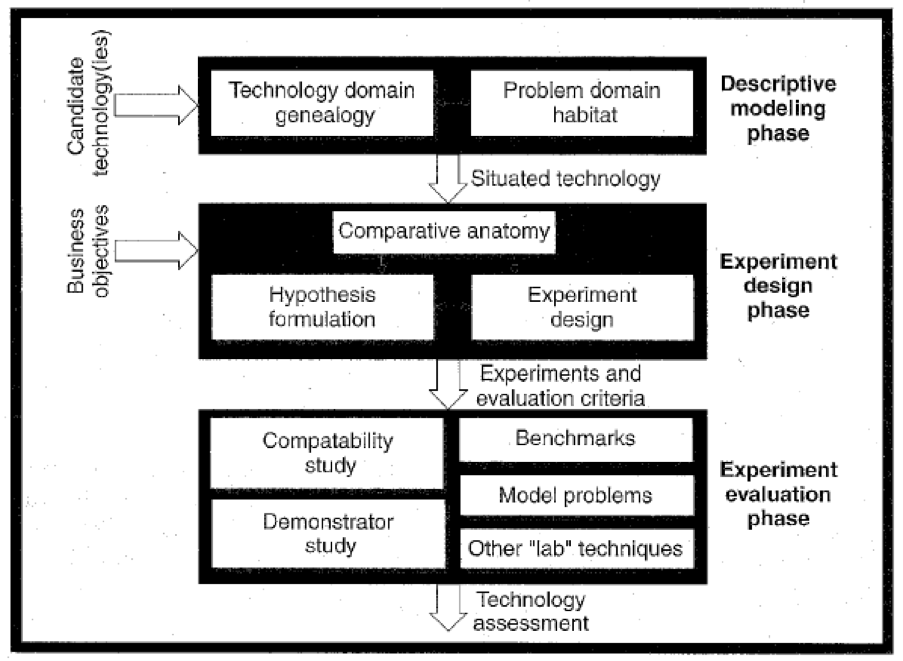
\includegraphics[scale=0.5]{figs/framework.png}
  \caption{Software technology evaluation framework.}
  \label{fig:framework}
\end{figure}


\section{Demonstrator Prototype}
\label{sec:design}

About 4 pages on:

\begin{enumerate}

\item An architectural overview of the application that has been implemented
\item High-level design, domain model, … (App assignment A)
\item May involve selected models from Chaps. 5 of the IoT and cloud books


\end{enumerate}

The example below shows how you may include code. There are similar
styles for many other langages - in case you do not use Java in your
project. You can wrap the listing into a figure in case you need to
refer to it. How to create a figure was shown in Section~\ref{sec:technology}.

\lstinputlisting[language=java]{code/BoksVolum.java}


\section{Prototype Implementation}
\label{sec:implementation}

This section should provide details of how the prototype has been implemented which may involve presentation of suitable code snippets.


\section{Test-bed Environment and Experiments}
\label{sec:evaluation}

About 2 pages that:

\begin{description}
\item[Explains] how the prototype has been tested the test-bed environment.

\item[Explains] what experiments have been done and the results.

\end{description}

For some reports you may have to include a table with experimental
results are other kinds of tables that for instance compares
technologies. Table~\ref{tab:results} gives an example of how to create a table.

\begin{table}
\centering
\begin{tabular}{llrrrrrr}
  Config & Property & States & Edges & Peak & E-Time & C-Time & T-Time
  \\ \hline \hline
22-2 & A   &    7,944  &   22,419  &  6.6  \%  &  7 ms & 42.9\% &  485.7\% \\
22-2 & A   &    7,944  &   22,419  &  6.6  \%  &  7 ms & 42.9\% &  471.4\% \\
30-2 & B   &   14,672  &   41,611  &  4.9  \%  & 14 ms & 42.9\% &  464.3\% \\
30-2 & C   &   14,672  &   41,611  &  4.9  \%  & 15 ms & 40.0\% &  420.0\% \\ \hline
10-3 & D   &   24,052  &   98,671  & 19.8  \%  & 35 ms & 31.4\% &  285.7\% \\
10-3 & E   &   24,052  &   98,671  & 19.8  \%  & 35 ms & 34.3\% &  308.6\% \\
\hline \hline
\end{tabular}
\caption{Selected experimental results on the communication protocol example.}
\label{tab:results}
\end{table}


\section{Conclusions}

Concludes on the project, including the technology, its maturity,
learning curve, and quality of the documentation.

The references used throughput the report should constitute a well
chosen set of references, suitable for someone interesting in learning
about the technology.


\bibliographystyle{plain}
\bibliography{report.bib}{}

\end{document}
